\section*{Lectura 4: Congruencias y Funtores.}

\begin{definition}
    Una \textbf{congruencia} es una categor\'ia $\Cc$ junto con una relaci\'on
    de equivalencia $\sim$ sobre morfismos de $\Cc$ definido tal que si $f \in
    \Hom{(A,B)}$, y $f \sim g$, entonces $g \in \Hom{(A,B)}$, y si $f \sim f'$ y
     $g \sim g'$, entonces $g \circ f \sim g' \circ f'$.
\end{definition}

\begin{figure}[h]
    \centering
    \[\begin{tikzcd}
	&&&&& {[f]} \\
	A &&&&&& B \\
	& {[g]}
	\arrow["{f_2}"{description}, curve={height=-6pt}, dashed, from=2-1, to=2-7]
	\arrow["{f_0}"{description}, curve={height=-30pt}, dashed, from=2-1, to=2-7]
	\arrow["{f_1}"{description}, curve={height=-18pt}, dashed, from=2-1, to=2-7]
	\arrow["{g_2}"{description}, curve={height=6pt}, squiggly, from=2-1, to=2-7]
	\arrow["{g_1}"{description}, curve={height=18pt}, squiggly, from=2-1, to=2-7]
	\arrow["{g_0}"{description}, curve={height=30pt}, squiggly, from=2-1, to=2-7]
\end{tikzcd}\]
    \caption{Una relaci\'on de equvalencia entre morfismos.}
    \label{fig_9}
\end{figure}

\begin{definition}
    Sea $\Cc$ una congruencia con relaci\'on de equivalencia  $\sim$. Definimos
    la  \textbf{categor\'ia cociente}, $\faktor{\Cc}{\sim}$ como la categor\'ia
    cuya objetos son los objetos de $\Cc$ y morfismos son las clases de
    equivalencias de  $\sim$. Si  $[f]:A \xrightarrow{} B$ es ub morfismo de
    $\faktor{\Cc}{\sim}$, entonces denotamos su conjunto como $[f] \in [A,B]$.
\end{definition}

\begin{theorem}\label{thm_4.4}
    Sea $\Cc$ una categor\'ia y $\sim$ una relaci\'on de equivalencia entre
    morfismos de $\Cc$. Entonces el coategor\'ia cociente  $\faktor{\Cc}{\sim}$
    es una categor\'ia.
\end{theorem}
\begin{proof}
    Nota que por definici\'on que $\obj{\faktor{\Cc}{\sim}}=\obj{\Cc}$, as\'i
    que por hipotesis, $\obj{\faktor{\Cc}{\sim}}$ es una clase. De igual manera,
    defina para todo $A,B \in \obj{\Cc}$, $[A,B]=\{[f] : f \in \Hom{(A,B)}\}$.
    Como $\Hom{(A,B)}$ es un conjunto para todo $A$ y $B$, y $\sim$ particiona
    el conjunto de todos los  $\Hom{(A,B)}$, entonces resulta que $[A,B]$ tiene
    que ser un conjunto tambien.

    Ahora sean $f$ y  $g$ morfismos de $\Cc$. Nota que por definici\'on de una
    congruencia, que como $f \sim f'$ y $g \sim g'$ implica que $g \circ f \sim
    g' \circ f'$, entonces la comopsici\'on  $[g] \circ [f]=[g \circ f]$ esta
    bien definido, si existe. Ahora sea $h$ un mrofismo. Entonces nota que
    $([g] \circ [f]) \circ [h]=[g \circ f] \circ [h]=[(g \circ f) \circ h]=[g
    \circ f \circ h]$ y $[g] \circ ([f] \circ [h])=[g] \circ [f \circ h]=[g
    \circ (f \circ h)]=[g \circ f \circ h]$. Entonces tenemos que $\circ$ es
    associativa si $([g] \circ [f]) \circ [h]$ \'o $[g] \circ ([f] \circ [h])$
    esta definida.

    Por ultimo, considere la identidad $1_A$ sobre el objeto  $A$. Entonces nota
    que  $[g] \circ [1_A]=[g \circ 1_A]=[g]$ y $[1_A] \circ [f]=[1_A \circ
    f]=[f]$; as\'i que $[1_A]$ es la identidad de $A$ en  $\faktor{\Cc}{\sim}$.
    As\'i que $\faktor{\Cc}{\sim}$ es una categor\'ia.
\end{proof}

\begin{figure}[h]
    \centering
    \[\begin{tikzcd}
	& {\faktor{\Cc}{\sim}} \\
	\\
	A &&&&&& B
	\arrow["{[f]}"{description}, curve={height=-30pt}, dashed, from=3-1, to=3-7]
	\arrow["{[g]}"{description}, curve={height=30pt}, squiggly, from=3-1, to=3-7]
\end{tikzcd}\]
    \caption{La categor\'ia cociente $\faktor{\Cc}{\sim}$, donde $\Cc$ es la
    categor\'ia de la figura \ref{fig_9}.}
    \label{}
\end{figure}

\begin{definition}
    Sea $\Ac$ y $\Cc$ dos categor\'ias. Un \textbf{funtor covariante} $T:\Ac
    \xrightarrow{} \Cc$ es una map definido tal que si $A \in \obj{\Ac}$,
    entonces $T(A) \in \obj{\Cc}$ y si $f:A \xrightarrow{} B$ es un morfismo en
    $\Ac$, entonces  $T(f):T(A) \xrightarrow{} T(B)$ es un morfismo en $\Cc$, y
    que $T(g \circ f)=T(g) \circ T(f)$ y $T(1_A)=1_{T(A)}$.
\end{definition}

\begin{figure}[h]
    \centering
    \[\begin{tikzcd}[sep=scriptsize]
	& \Ac &&&&&&&&&& \Cc \\
	A && A && B &&&& {T(A)} && {T(A)} && {T(B)} \\
	\\
	&&&& C &&&&&&&& {T(C)}
	\arrow["g", from=2-5, to=4-5]
	\arrow[""{name=0, anchor=center, inner sep=0}, "f", from=2-3, to=2-5]
	\arrow["{g \circ f}"', from=2-3, to=4-5]
	\arrow["{1_A}"', from=2-3, to=2-1]
	\arrow["{T(f)}", from=2-11, to=2-13]
	\arrow["{T(g)}", from=2-13, to=4-13]
	\arrow["{T(g) \circ T(f)}"', from=2-11, to=4-13]
	\arrow[""{name=1, anchor=center, inner sep=0}, "{1_{T(A)}}", from=2-11, to=2-9]
	\arrow["T", curve={height=-18pt}, shorten <=40pt, shorten >=40pt, Rightarrow, from=0, to=1]
\end{tikzcd}\]
    \caption{Un funtor $T$ covariante entre dos diagramas commutativas bajo las
    categor\'ias $\Ac$ y $\Cc$.}
    \label{fig_11}
\end{figure}

\begin{definition}
    Sea $\Ac$ y $\Cc$ dos categor\'ias. Un \textbf{funtor contravariante} $S:\Ac
    \xrightarrow{} \Cc$ es una map definido tal que si $A \in \obj{\Ac}$,
    entonces $S(A) \in \obj{\Cc}$ y si $f:A \xrightarrow{} B$ es un morfismo en
    $\Ac$, entonces  $S(f):T(B) \xrightarrow{} T(A)$ es un morfismo en $\Cc$, y
    que $T(g \circ f)=T(f) \circ T(g)$ y $T(1_A)=1_{T(A)}$.
\end{definition}

\begin{figure}[h]
    \centering
    \[\begin{tikzcd}[sep=scriptsize]
	& \Ac &&&&&&&&&& \Cc \\
	A && A && B &&&& {S(A)} && {S(A)} && {S(B)} \\
	\\
	&&&& C &&&&&&&& {S(C)}
	\arrow["g", from=2-5, to=4-5]
	\arrow[""{name=0, anchor=center, inner sep=0}, "f", from=2-3, to=2-5]
	\arrow["{g \circ f}"', from=2-3, to=4-5]
	\arrow["{1_A}"', from=2-3, to=2-1]
	\arrow["{S(f)}"', from=2-13, to=2-11]
	\arrow["{S(g)}"', from=4-13, to=2-13]
	\arrow["{S(f) \circ S(g)}", from=4-13, to=2-11]
	\arrow[""{name=1, anchor=center, inner sep=0}, "{1_{S(A)}}"', from=2-9, to=2-11]
	\arrow["S", curve={height=-18pt}, shorten <=40pt, shorten >=40pt, Rightarrow, from=0, to=1]
\end{tikzcd}\]
    \caption{Un funtor $S$ contravariante entre dos diagramas commutativas bajo
        las categor\'ias $\Ac$ y $\Cc$.}
    \label{fig_12}
\end{figure}

\begin{example}\label{}
    \begin{enumerate}
        \item[(1)] Considere el funtor $F:\Top \xrightarrow{} \Conj$ tal que
            s\'i $X$ es un espacio topol\'ogico, entonces  $T(X)=X$ como
            conjunto general y s\'i $f:X \xrightarrow{} Y$ es una mapa continua,
            entonces $T(f):X \xrightarrow{} Y$ es una mapa general. Es decir
            este funtor lleva los espacios topologicos los funciones continuas a
            si mismos, pero quitando las nociones de topolog\'ia. Este funtor es
            covariante, y se llama el \textbf{funtor olvidadizo}.

        \item[(2)] El \textbf{funtor identidad} $J:\Cc \xrightarrow{} \Cc$ es el
            funtor que lleva objetos de $\Cc$ a si mismos, y morfismos de $\Cc$
            a si mismos. Es decir, no cambia la categor\'ia.

        \item[(3)] Sea $M$ un espacio topol\'ogico. Defina  $T_m:\Top
            \xrightarrow{} \Top$ definida por $T_M:X \xrightarrow{} X \times M$
            en el topologia producto, y $T_M:f \xrightarrow{} f \times 1_M$,
            para cualquier mapa continua $f:X \xrightarrow{} Y$. Entonces $T_m$
            es un funtor covariante.
    \end{enumerate}
\end{example}

\begin{definition}
    Definimos una \textbf{equivalencia} de una categor\'ia $\Cc$ de ser un
    morfismo  $f:A \xrightarrow{} B$ para lo cual existe un morfismo $g:B
    \xrightarrow{} A$ tal que $g \circ g=1_B$ y  $g \circ f=1_A$.
\end{definition}

\begin{example}\label{}
    Los equivalencias de la categor\'ia $\Top$ son los homeomorfismos, y las
    equivalencias de  $\Grp$ son los isomorfismos.
\end{example}

\begin{theorem}\label{thm_4.5}
    Sean $\Ac$ y  $\Cc$ categor\'ias y  $T:\Ac \xrightarrow{} \Cc$ una functor.
    Entonces s\'i $f$ es una equivalencia en  $\Ac$, entonces  $T(f)$ es una
    equivalencia en $\Cc$.
    \[\begin{tikzcd}
	A && B &&& {T(A)} && {T(B)} \\
	\\
	\\
	A && B &&& {S(A)} && {S(B)}
	\arrow[""{name=0, anchor=center, inner sep=0}, "f", curve={height=-6pt}, from=1-1, to=1-3]
	\arrow["h", curve={height=-6pt}, from=1-3, to=1-1]
	\arrow[""{name=1, anchor=center, inner sep=0}, "{T(f)}", curve={height=-6pt}, from=1-6, to=1-8]
	\arrow["{T(h)}", curve={height=-6pt}, from=1-8, to=1-6]
	\arrow[""{name=2, anchor=center, inner sep=0}, "f", curve={height=-6pt}, from=4-1, to=4-3]
	\arrow["h", curve={height=-6pt}, from=4-3, to=4-1]
	\arrow[""{name=3, anchor=center, inner sep=0}, "{S(f)}"', curve={height=6pt}, from=4-8, to=4-6]
	\arrow["{S(h)}"', curve={height=6pt}, from=4-6, to=4-8]
	\arrow["T", curve={height=-18pt}, shorten <=33pt, shorten >=33pt, Rightarrow, from=0, to=1]
	\arrow["S", curve={height=-18pt}, shorten <=33pt, shorten >=33pt, Rightarrow, from=2, to=3]
\end{tikzcd}\]
\end{theorem}
\begin{proof}
    Suponga primero que $T$ es covariante. Es decir que para cualquier morfismo
     $f:A \xrightarrow{} B$, $T(f):T(A) \xrightarrow{} T(B)$ lleva a $T(A)$ a
     $T(B)$, y $T(g \circ f)=T(g) \circ T(f)$. Ahora suponga que $f:A
     \xrightarrow{} B$ es una equvalencia en $\Ac$. Entonces existe un morfismo
     $h:B \xrightarrow{} A$ tal que $h \circ f=1_B$ y  $f \circ h=1_A$.
     Entonoces  $T(h \circ f)=T(h) \circ T(f)=1_{T(B)}$ y $T(f \circ h)=T(f)
     \circ T(h)=1_{T(A)}$. Entonces por definici\'on, podemos ver que $T(f)$ es
     una equivalencia en $\Cc$.

     De igual forma de  $T$ se contravariante, la demostraci\'on procede el
     mismo manera, con la diferencia que notamos que $T(f):T(B) \xrightarrow{}
     T(A)$ lleva a $T(B)$ a $T(A)$ para todo $f:A \xrightarrow{} B$ y que $T(g
     \circ f)=T(f) \circ T(g)$.
\end{proof}

\begin{definition}
    Sean $X$ y  $Y$ espacios topologicos, y sean  $f_0:X \xrightarrow{} Y$ y
    $f_1:X \xrightarrow{} Y$ mapas continuas. Decimos que $f_0$ es
    \textbf{homot\'opico} a $f_1$ s\'i existe una mapa continua $F:X \times I
    \xrightarrow{} Y$ tal que $F(x,0)=f_0(x)$ y $F(x,1)=f_1(x)$ para todo $X \in
    X$. Decimos que  $f_0$ y $f_1$ son \textbf{homot\'opicos} y escribimos $f_0
    \simeq f_1$.
\end{definition}

\begin{figure}[h]
    \centering
    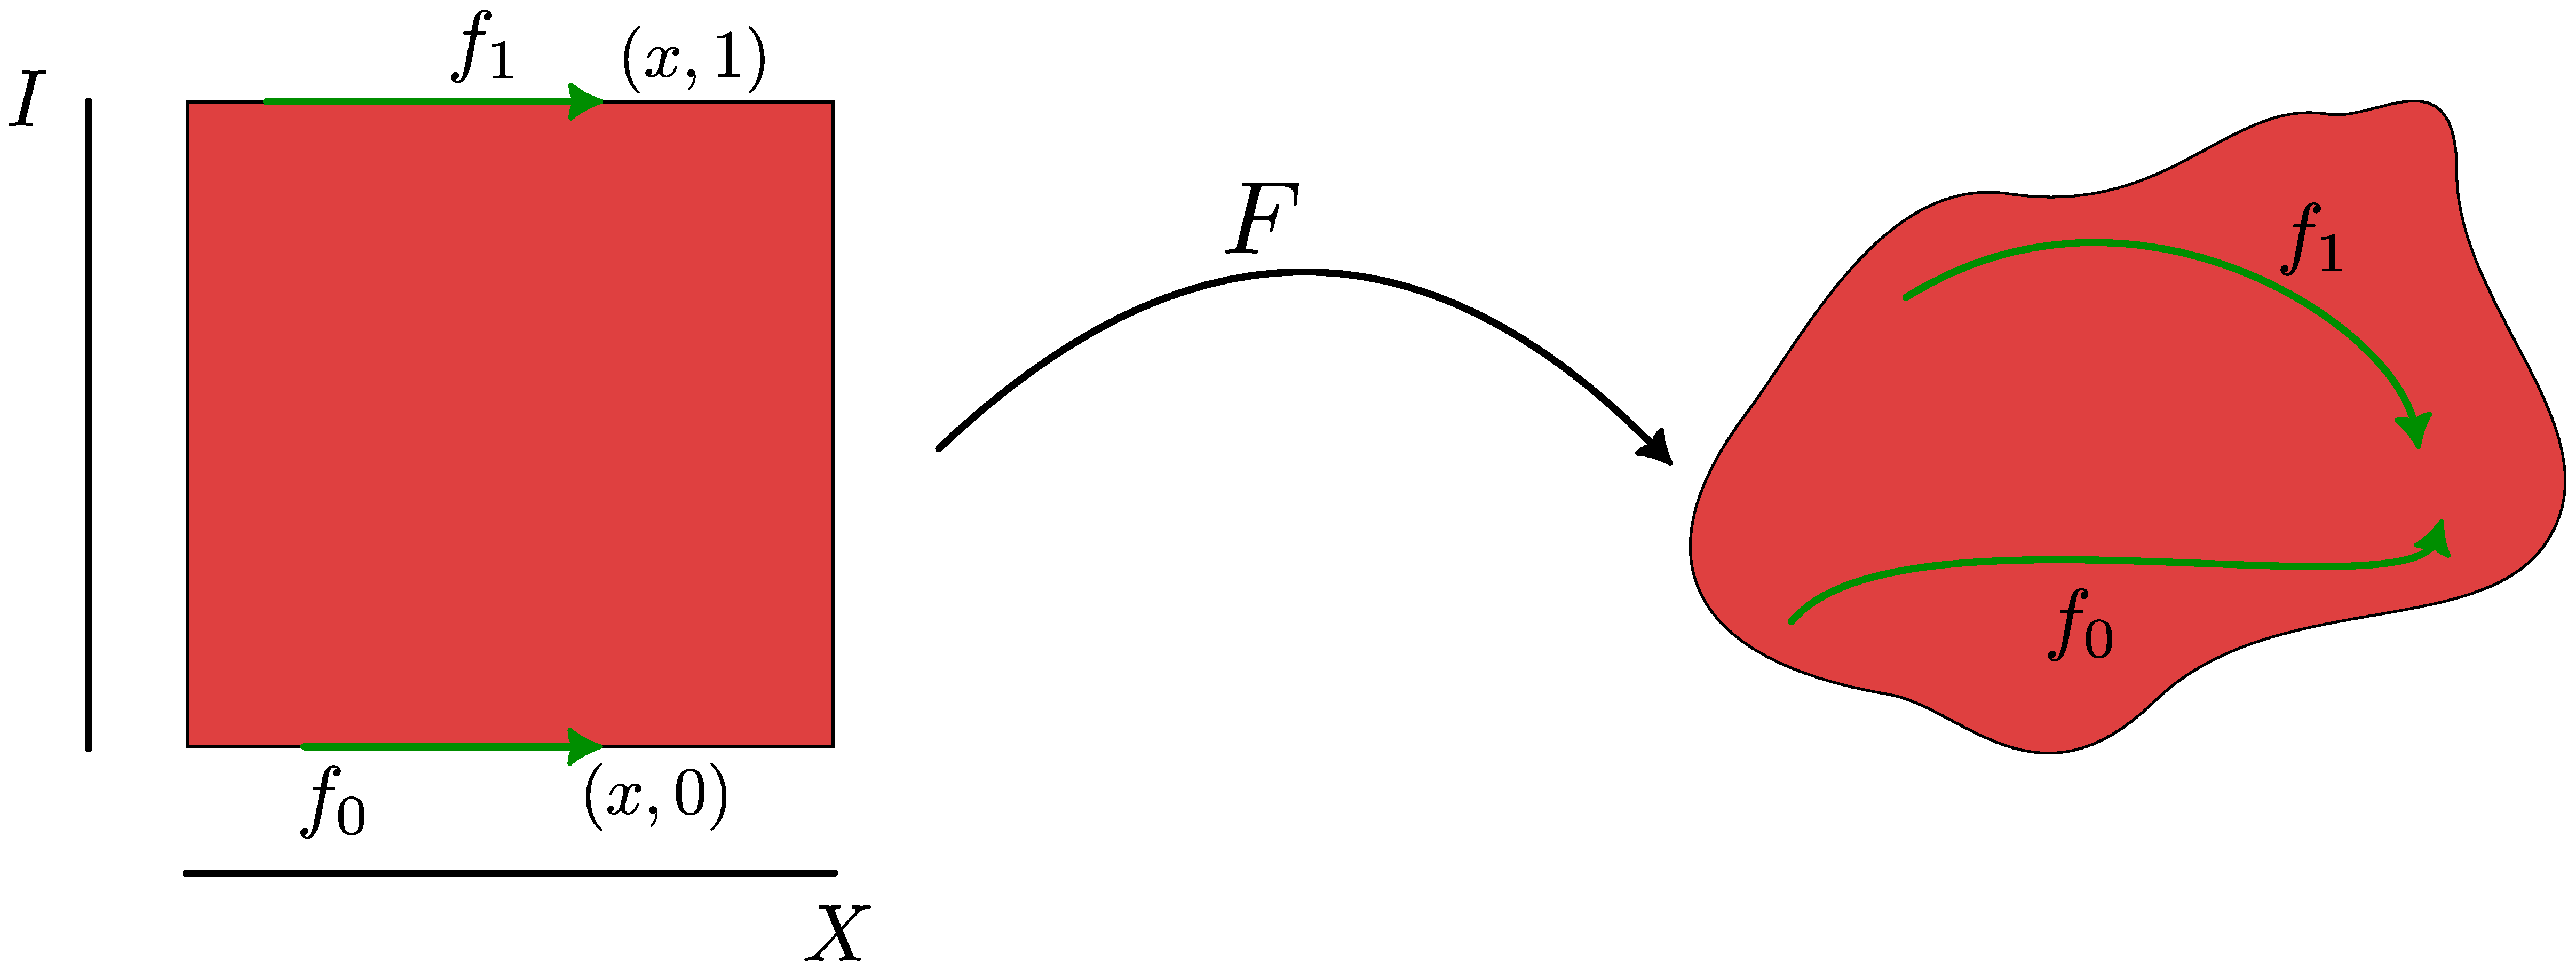
\includegraphics[scale=0.2]{Figures/homotopia.eps}
    \caption{Dos mapas continuas $f_0$ y $f_1$ homot\'opicos.}
    \label{fig_13}
\end{figure}
